

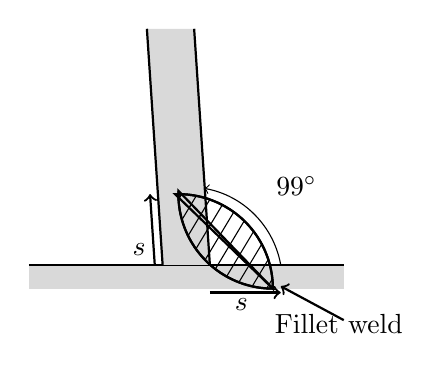
\begin{tikzpicture}

    % Draw the horizontal base plate
    \fill[gray!30] (-2,0) rectangle (2,-0.3); % Shaded base plate
    \draw[thick] (-2,0) -- (2,0);

    % Draw the vertical plate
    \fill[gray!30] (-0.3,0) -- (-0.5,3) -- (0.1,3) -- (0.3,0) -- cycle; % Shaded vertical plate
    \draw[thick] (-0.3,0) -- (-0.5,3); % Left side
    \draw[thick] (0.3,0) -- (0.1,3); % Right side
	\draw[thick][->] (-0.4,0) -- (-0.46,0.9);
	\draw[thick][->] (0.3,-0.35) -- (1.2,-0.35);
	\draw[thick][->] (2,-0.7) -- (1.2,-0.27);


    % Draw the fillet weld area
  \begin{scope}
    % Clip to the arc shape
    \clip (1.1,-0.3) arc[start angle=0, end angle=92, radius=1.2cm] -- (1.1,-0.3) -- cycle;
    % Draw diagonal lines
    \foreach \x in {-2,-1.8,...,3} { % Adjust spacing as needed
        \draw[thin] (\x,-2) -- (\x+3,3); % Adjust slope and coverage as needed
    }
\end{scope}

% Outline the arc
\draw[thick] (1.1,-0.3) arc[start angle=0, end angle=92, radius=1.2cm] -- (1.1,-0.3) -- cycle;
    \draw[thick] (1.1,-0.3) arc[start angle=0, end angle=92, radius=1.2cm];
	\draw[thick] (1.1,-0.3) arc[start angle=270, end angle=178, radius=1.2cm];
\begin{scope}
    % Clip to the arc shape
    \clip (1.1,-0.3) arc[start angle=270, end angle=178, radius=1.2cm] -- (1.1,-0.3) -- cycle;
    % Draw diagonal lines
    \foreach \x in {-2,-1.8,...,3} { % Adjust spacing as needed
        \draw[thin] (\x,-2) -- (\x+3,3); % Adjust the slope and coverage of the lines
    }
\end{scope}

% Outline the arc shape
\draw[thick] (1.1,-0.3) arc[start angle=270, end angle=178, radius=1.2cm] -- (1.1,-0.3) -- cycle;
    % Draw the angle label
    \draw[->] (1.2,0) arc[start angle=10, end angle=80, radius=1.2cm];
    \node at (1.4,1) {$99^\circ$};

    % Label 's' for the fillet weld throat thickness
    \node at (0.7,-0.5) {$s$};
    \node at (-0.6,0.2) {$s$};

    % Label for "Fillet weld"
    \node[below right] at (1,-0.5) {Fillet weld};

\end{tikzpicture}

